\subsubsection{Ambiente de teste}

\indent \qquad Todos os tempos foram medidos na mesma máquina: um notebook com
processador Intel Core i7-13620H de 13ª geração e 15,7 GB de memória, sob
Windows 11 Home. O programa foi compilado com o gcc 13.2.0 (MinGW-W64), usando
as opções \texttt{-std=c99 -O2 -Wall}. A medição emprega a função
\texttt{clock()}, da biblioteca \texttt{time.h}, e o cronômetro envolve apenas a
chamada do \texttt{insertionSort}: a geração da instância e a gravação dos
arquivos de entrada, de saída e de tempo ficam de fora da conta. Cada uma das
dezoito combinações foi executada uma única vez.

\subsubsection{Tempos medidos}

\indent \qquad A Tabela \ref{tab:tempos_insertion} reúne os tempos obtidos para
os seis tamanhos de entrada e os três tipos de instância exigidos pelo trabalho.

\begin{spacing}{1.0}
	\begin{table}[H]
		\centering
		\caption{Tempo de ordenação do Insertion Sort, em segundos, nas dezoito combinações de tamanho e tipo de entrada.}
		\label{tab:tempos_insertion}
		\renewcommand{\arraystretch}{1.2}
		\begin{tabular}{rrrr}
			\toprule
			\textbf{n} & \textbf{Crescente} & \textbf{Decrescente} & \textbf{Random} \\
			\midrule
			10 & 0,000000 & 0,000000 & 0,000000 \\
			100 & 0,000000 & 0,000000 & 0,000000 \\
			1.000 & 0,000000 & 0,000000 & 0,000000 \\
			10.000 & 0,000000 & 0,012000 & 0,008000 \\
			100.000 & 0,000000 & 1,276000 & 0,613000 \\
			1.000.000 & 0,000000 & 119,339000 & 59,224000 \\
			\bottomrule
		\end{tabular}
	\end{table}
\end{spacing}

\subsubsection{Gráfico dos tempos}

\indent \qquad A Figura \ref{fig:grafico_insertion} mostra os mesmos tempos em
forma de curva. As três séries partem do zero e assim permanecem até $n =
1.000$; a partir daí, a decrescente e a aleatória sobem juntas e guardam entre
si uma distância que não muda até o último ponto, com a decrescente sempre acima
da aleatória e sempre pela mesma proporção. A crescente não sai do zero em
nenhum dos seis tamanhos, e por isso acompanha o eixo horizontal de ponta a
ponta.

\begin{figure}[H]
	\centering
	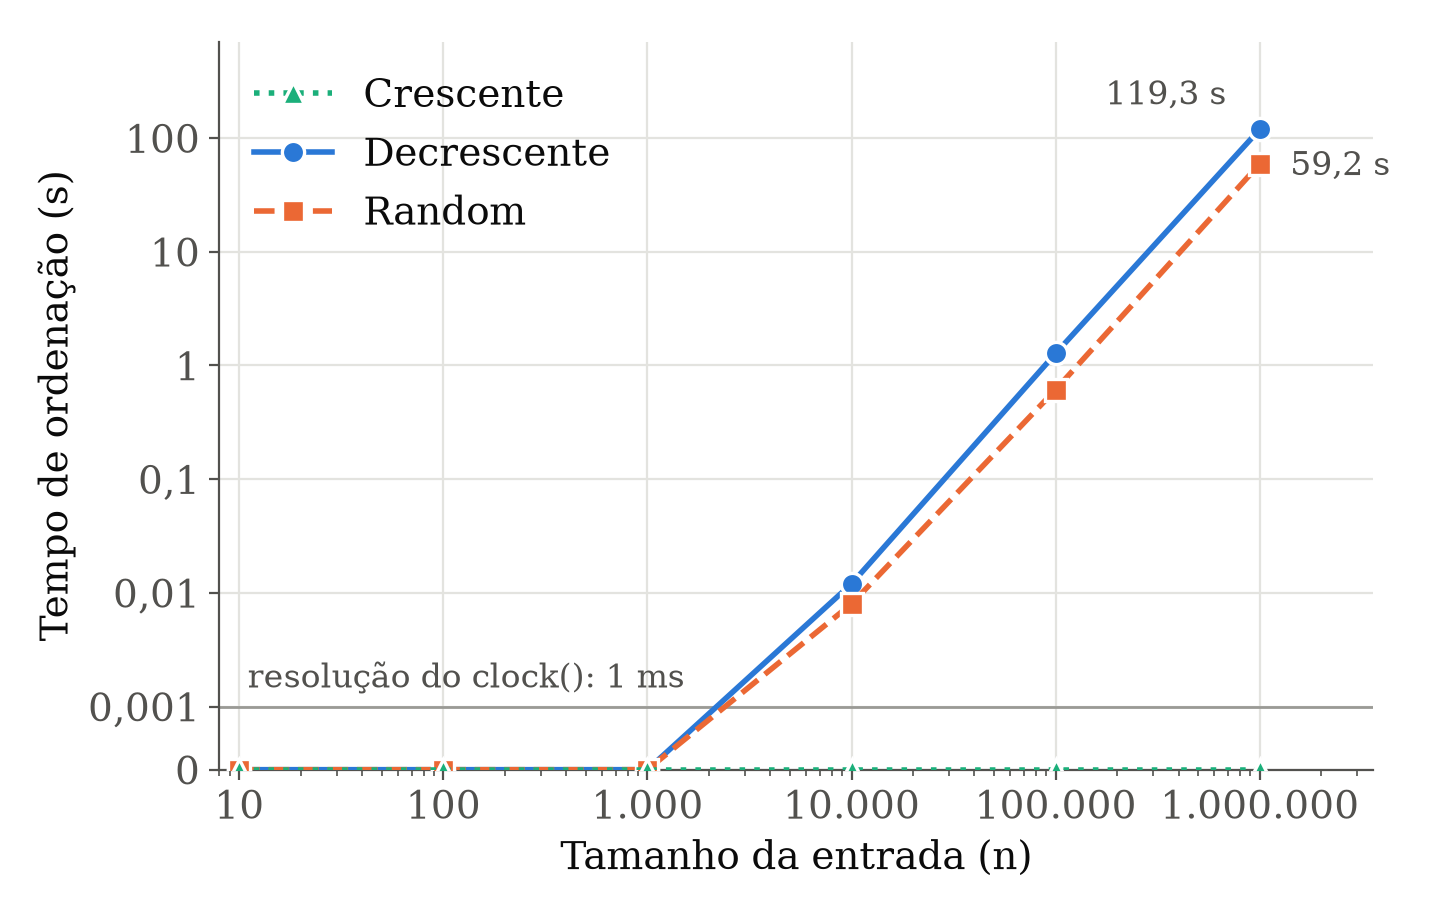
\includegraphics[width=0.95\textwidth]{Imagens/Insertion Sort/grafico.png}
	\caption{Tempo de ordenação em função do tamanho da entrada. O eixo do tempo é logarítmico acima de um milissegundo e linear abaixo disso, o que permite representar no gráfico as dez medições nulas.}
	\label{fig:grafico_insertion}
\end{figure}

\subsubsection{Discussão dos resultados}

\indent \qquad Os resultados confirmam o que a análise da Seção
\ref{sec:analise_insertion} previa. A entrada crescente, que é o melhor caso,
não registra tempo em nenhum tamanho: com o vetor já ordenado o laço interno
nunca executa, e o custo linear fica abaixo do que o relógio consegue medir. A
decrescente e a aleatória são ambas quadráticas --- multiplicar $n$ por dez
multiplicou o tempo por cerca de cem nas duas --- e a diferença entre elas está
apenas na constante: a decrescente, que é o pior caso, custa o dobro da
aleatória em todos os tamanhos medidos, porque cada elemento atravessa o trecho
ordenado inteiro em vez de metade dele.

\qquad Os dez valores iguais a zero na tabela não são falha de medição. Nesta
máquina, a função \texttt{clock()} só distingue variações a partir de um
milissegundo, e tudo o que roda mais rápido que isso é registrado como zero. É
o caso da coluna Crescente inteira e dos três menores tamanhos das outras duas
colunas.

\qquad O quadro geral é o de um algoritmo cujo desempenho depende mais da ordem
da entrada do que do seu tamanho. Para vetores pequenos, ou já quase ordenados,
o Insertion Sort é rápido o bastante para nem ser medido. Para vetores grandes
em ordem qualquer, ele deixa de ser viável: com 1.000.000 de elementos, o mesmo
código ou não registra tempo algum ou gasta quase dois minutos, e o que separa
os dois extremos é apenas a disposição inicial dos números.
